\chapter{設計}
\label{chap:sekkei}

本章では手書きベースWikiの要件と設計について述べる。

\newpage

\section{要件}
前章で示した手書きメモ・イラストを扱う既存のシステムの問題点を踏まえて、本システムの要件を整理する。
\begin{itemize}
    \item 手書きメモ・イラストを作成・編集できる\\
    タッチやスタイラスペンに対応したエディタを備え、手書きメモ・イラストを手軽に作成・編集することができる。
    \item 手書きメモ・イラストにハイパーリンクを追加できる\\
    作成した手書きメモ・イラスト同士の相互リンクを簡単な操作で定義できる。またメモ・イラストそのものも
    URLによって共有できる。
    \item 関連する手書きメモ・イラストを参照できる\\
    メモに追加されたリンク情報をに基づいて関連するメモ・イラストを
    推薦し、一覧できるよう表示する。
\end{itemize}
この要件を満たす手書きベースWikiのプロトタイプとしてDrawWikiを開発した。

\section{DrawWiki}
DrawWikiは本研究において開発した、手書きベースWikiのコンセプトを元にしたプロトタイプとなるアプリケーションである。(図\ref{drawwiki})
本章ではその主要な機能を使い方とともに解説する。

\begin{figure}[htbp]
    \begin{center}
        \fbox {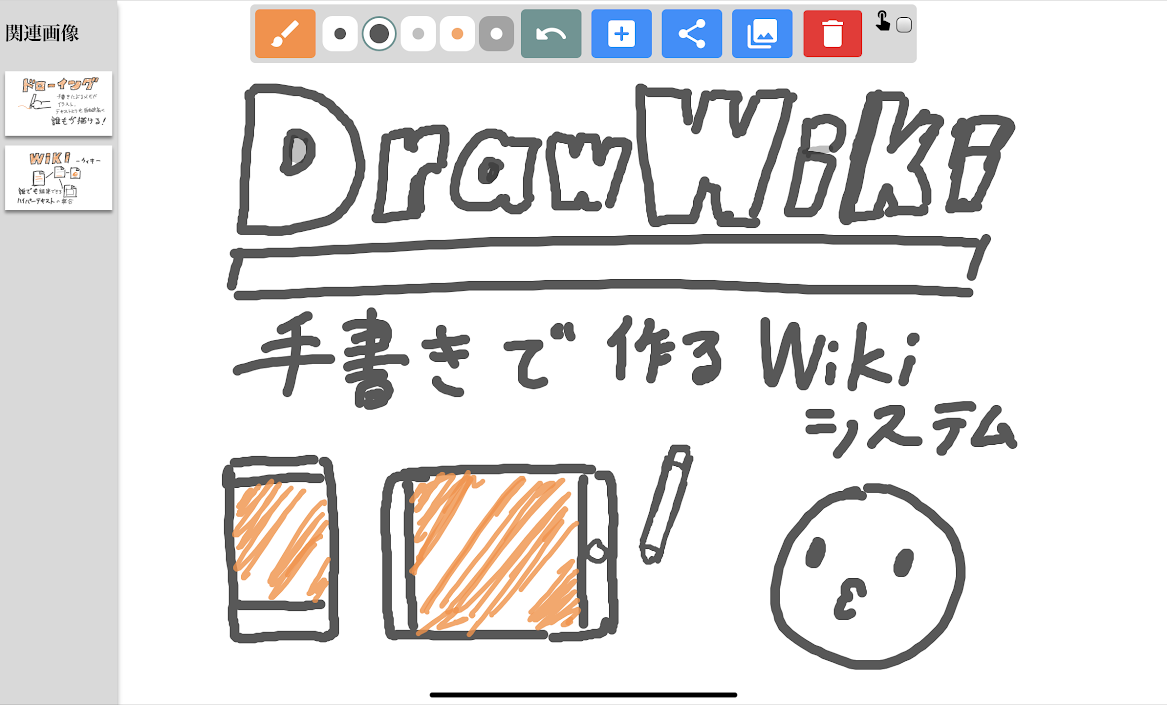
\includegraphics[width=100mm]{images/drawwikitop.png}} \end{center}
    \caption{DrawWikiの画面}
    \label{drawwiki}
\end{figure}

\subsection{DrawWikiの仕様}
DrawWikiにおける手書きメモ・イラストはSVG\cite{aboutsvg}形式で記録される。
SVGはXML\footnote{https://www.w3.org/XML/}をベースとする画像ファイルフォーマットであり、
手書きメモ・イラストをハイパーテキストとして扱う上で有利な以下のような特徴を持つ。
\begin{itemize}
    \item グラフィカルな表現を前提に設計されている\\
    SVGには曲線等を表現するPath要素や閉じた図形を表現するPolygon要素等の仕様が標準で備わっている。
    スタイラスから得られるデータをPath要素の属性として定義することで手書きのストロークを表現することができる。
    (例えばソースコード\ref{code:tegakipathcode}で図\ref{fig:tegakipath}のように表現できる)
    \item 構造を保持できる\\
    ラスターイメージと異なりSVGの実体は構造化されたテキストファイルであり、線分や点はピクセルではなく
    独立した要素として記述される。これにより書き順や編集履歴等の構造も保持され、再編集性が高い。
    \item ハイパーリンクを埋め込める\\
    SVGではXLink\footnote{https://www.w3.org/TR/xlink/}形式のハイパーリンクを任意の要素に埋め込むことができるため
    画像の中の個別の要素に対して複数のリンクを定義することができる。
    \item Web標準の技術である\\
    SVGは特定の企業の製品ではなく、その仕様は全て公開されている。また作成や表示に特別なソフトウェアを必要とせず、
    ブラウザがあれば閲覧することができる。
\end{itemize}

\begin{figure}[htbp]
    \begin{center}
        \fbox {
\includegraphics[width=70mm]{images/svgpath.png}} \end{center}
    \caption{SVG上で表現される手書きストローク} \label{fig:tegakipath}
\end{figure}

\begin{lstlisting}[caption=図\ref{fig:tegakipath}の実体, label=code:tegakipathcode]
    <path stroke-linejoin="round" stroke-linecap="round" stroke="#585858"
    stroke-width="10" class="" pointer-events="auto" fill="rgba(0,0,0,0)"
    id="1072-528" d="M 919 564 ,L 919 563 ,L 919 562 ,L 919 560 ,L 919 559 ... L 1064 520 "></path>
\end{lstlisting}


\subsection{機能と使い方}

\subsubsection{手書きメモ・イラストの作成・編集}

画面中央部分に自由に手書きができるキャンバスが配置されており、ここに描いたものが自動的に保存・アップロードされる。
一度アップロードしたメモ・イラストにはURLが割り振られるためWebを通じて他のユーザーが閲覧し、編集することもできる。
\\
既存の手書きメモアプリケーションと同様に、Redo等の編集支援機能を利用できるほか、
DrawWikiでは金箱らによるスケッチ技法Interactive Sketch\cite{130004638060}に基づいたコンパクトなブラシプリセット構成を採用している。
このスケッチ技法は以下の4種類のブラシを用いる
\begin{enumerate}
    \item 通常のペンで全体を描く
    \item 影や質感をグレーで表現する
    \item 輪郭を太い線で縁取る
    \item 特徴的な部分、機能を有する箇所をキーカラーでハイライトする
\end{enumerate}
これによりWikiとして活用する上で有利な以下のような特徴を持つ(図\ref{fig:interactivesketch})。
\begin{itemize}
    \item 太線で図のアウトラインが強調されるためサムネイル状態での視認性が確保される
    \item キーカラーによる強調表示でアイデアが伝わりやすくなる
    \item ブラシによって描き方がある程度統一され、スケッチ技量の巧拙を吸収できる
\end{itemize}

\begin{figure}[htbp]
    \begin{center}
        \fbox {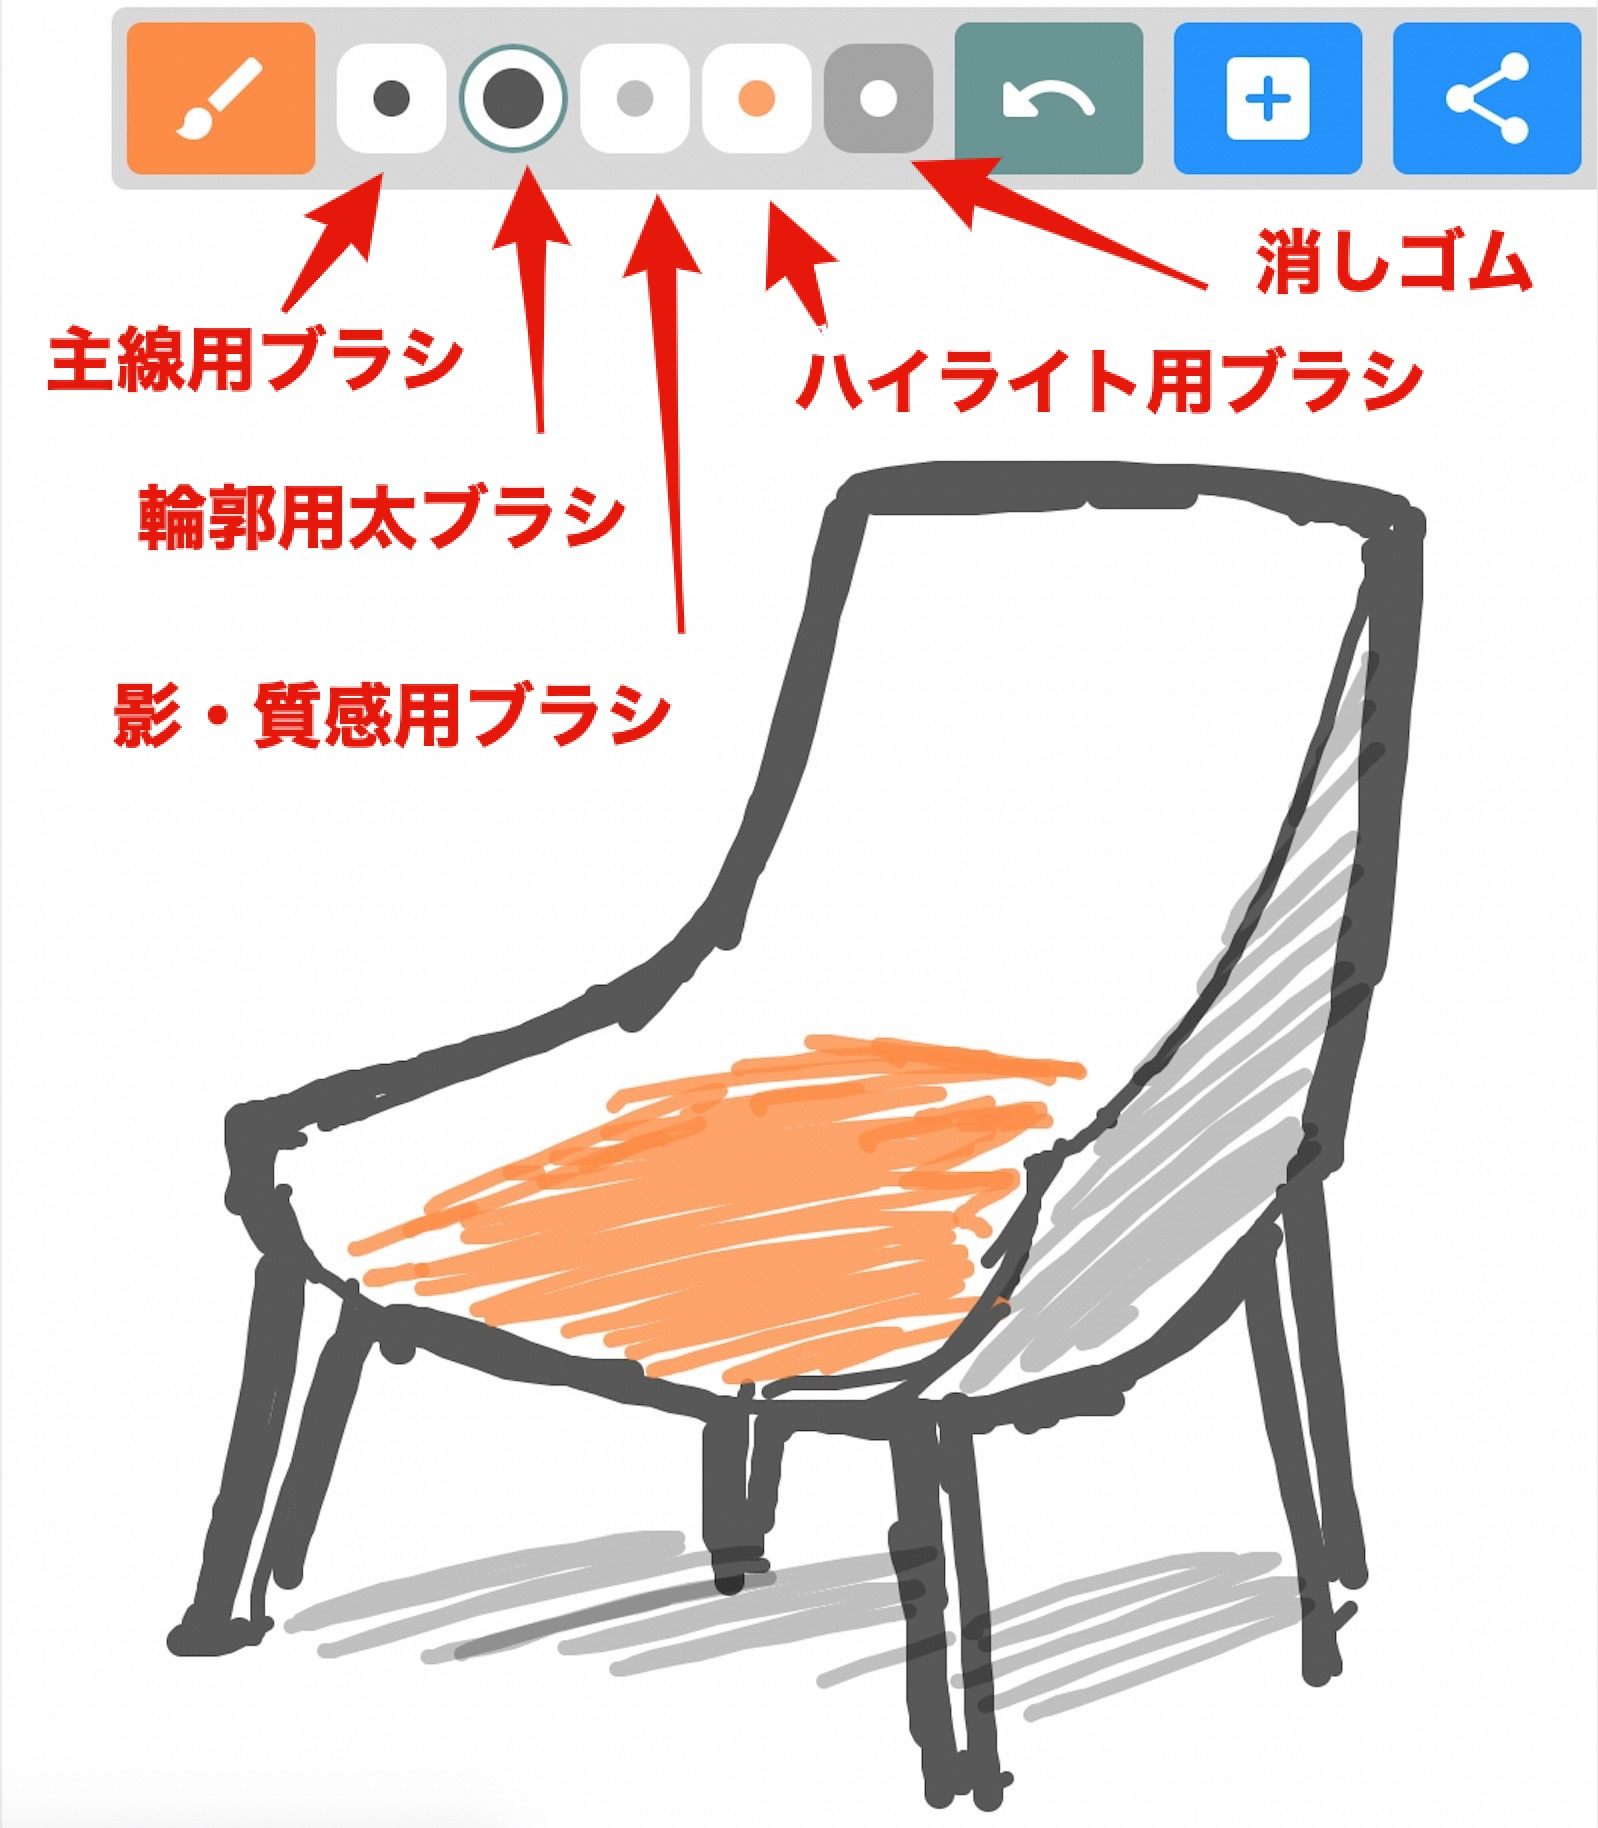
\includegraphics[width=60mm]{images/interactivesketch.jpg}} \end{center}
    \caption{プリセットを用いて描かれた図}
    \label{fig:interactivesketch}
\end{figure}

\subsubsection{ハイパーリンク埋め込み機能}

\begin{figure}[H] \begin{minipage}{0.5\hsize}
                         \begin{center} \fbox {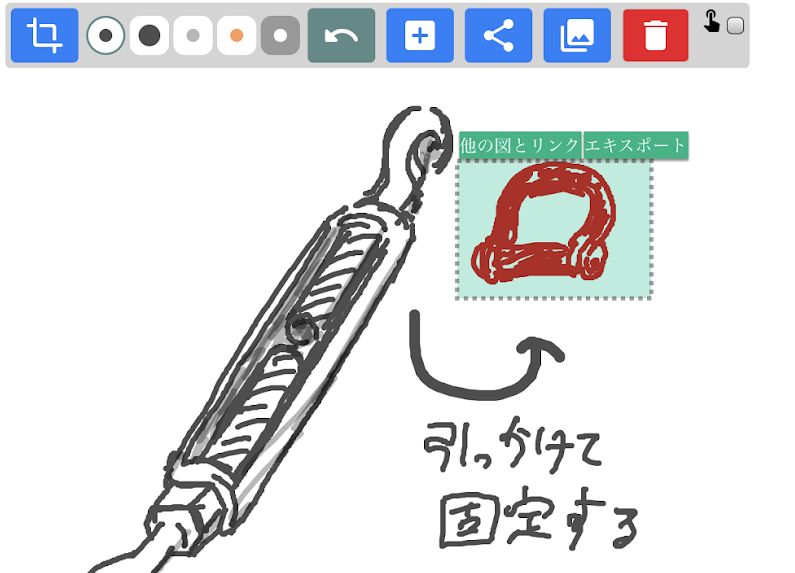
\includegraphics[width=70mm]{images/addLink1.png}}
                         \end{center} \caption{範囲選択ツール} \label{fig:addLink1}
\end{minipage} \begin{minipage}{0.5\hsize}
                   \begin{center} \fbox {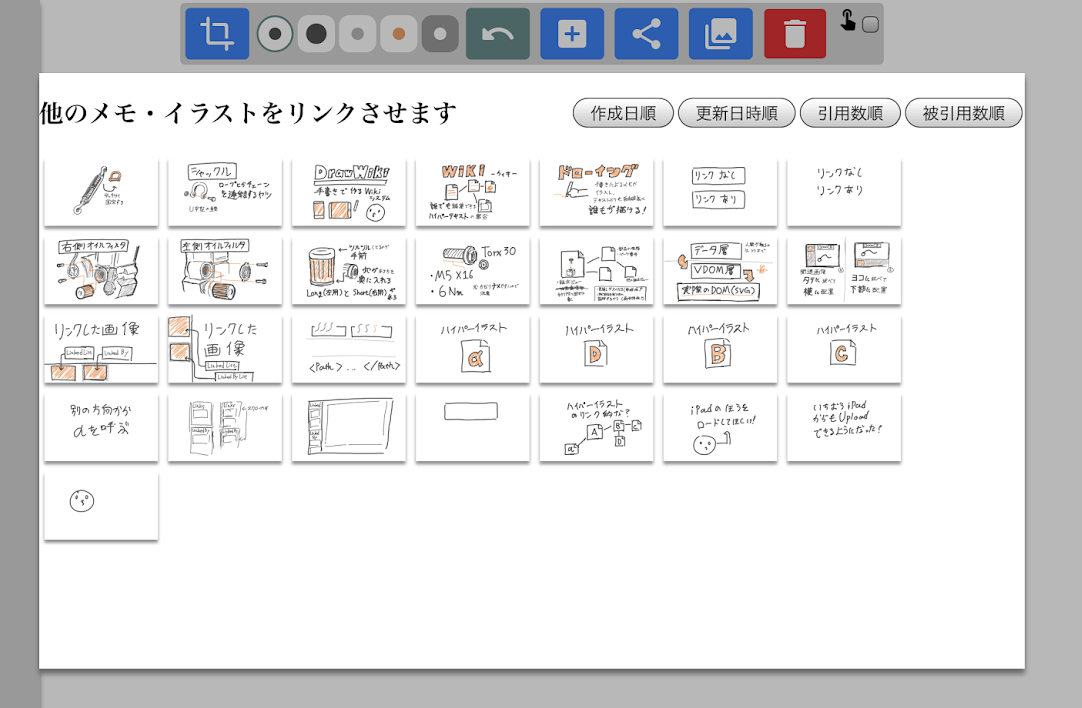
\includegraphics[width=70mm]{images/addLink2.png}}
                   \end{center} \caption{リンク埋め込み機能の操作画面} \label{fig:addLink2}
\end{minipage}
\end{figure}

範囲選択ツールを用いてハイパーリンクを埋め込みたい要素を選択することができる。
要素を選択して"他の図とリンクボタン"を押すと今まで作成したメモ・イラストの一覧がダイアログで表示され、
その中からリンクさせたい図を選ぶとその図へのハイパーリンクが要素に埋め込まれる。

\subsubsection{関連画像の表示機能}

\begin{figure}[htbp] \begin{minipage}{0.5\hsize}
                         \begin{center} \fbox {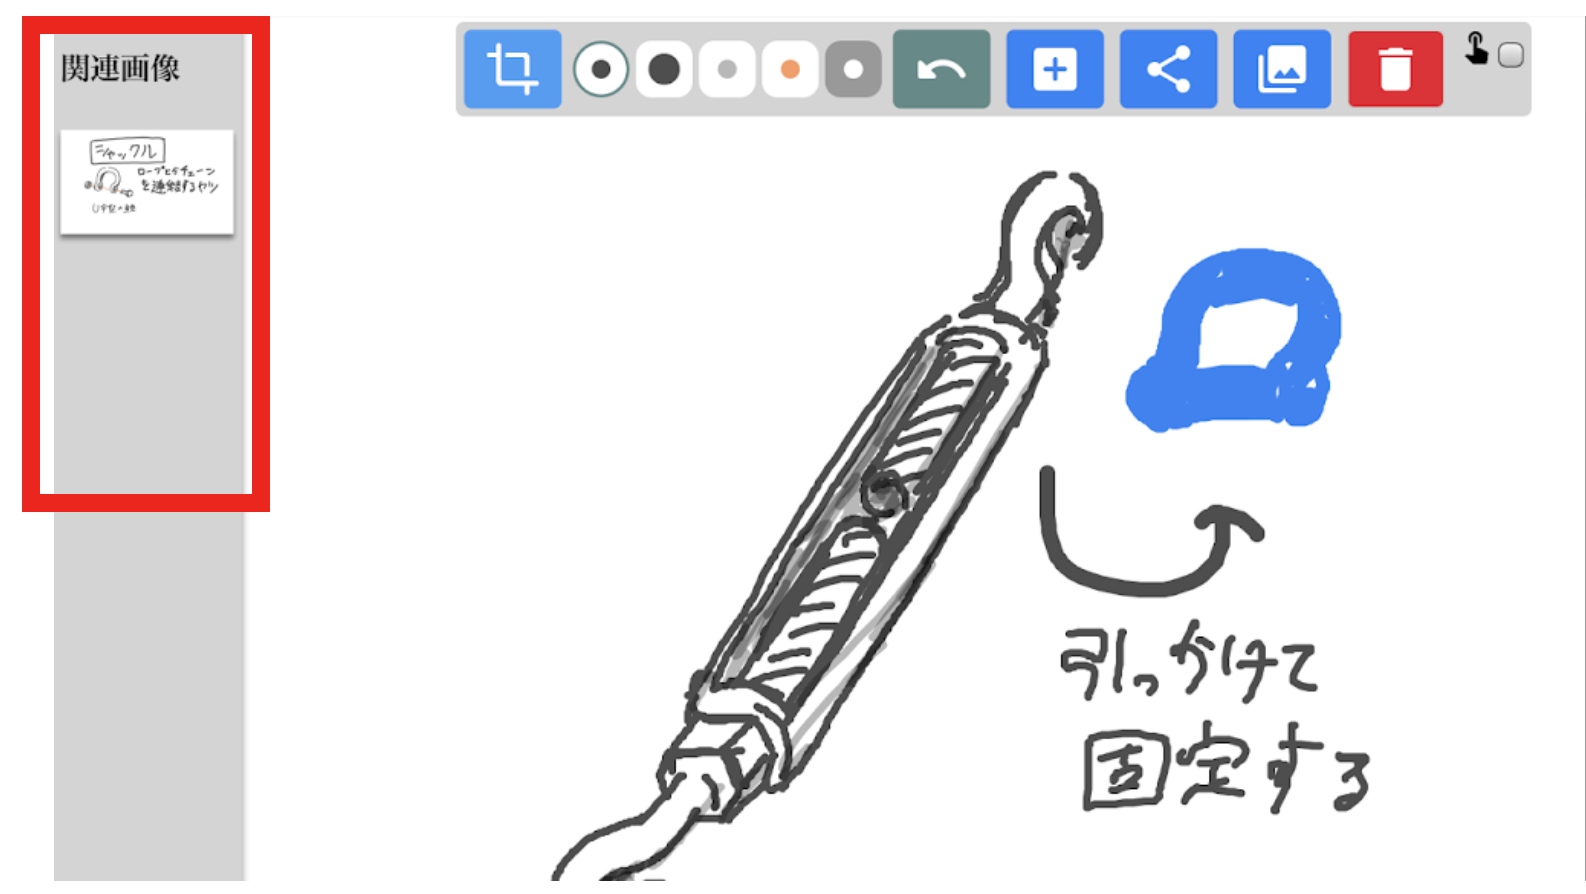
\includegraphics[width=70mm]{images/addLink3.png}}
                         \end{center} \caption{関連画像の表示機能} \label{fig:linkedIllust1}
\end{minipage} \begin{minipage}{0.5\hsize}
                   \begin{center} \fbox {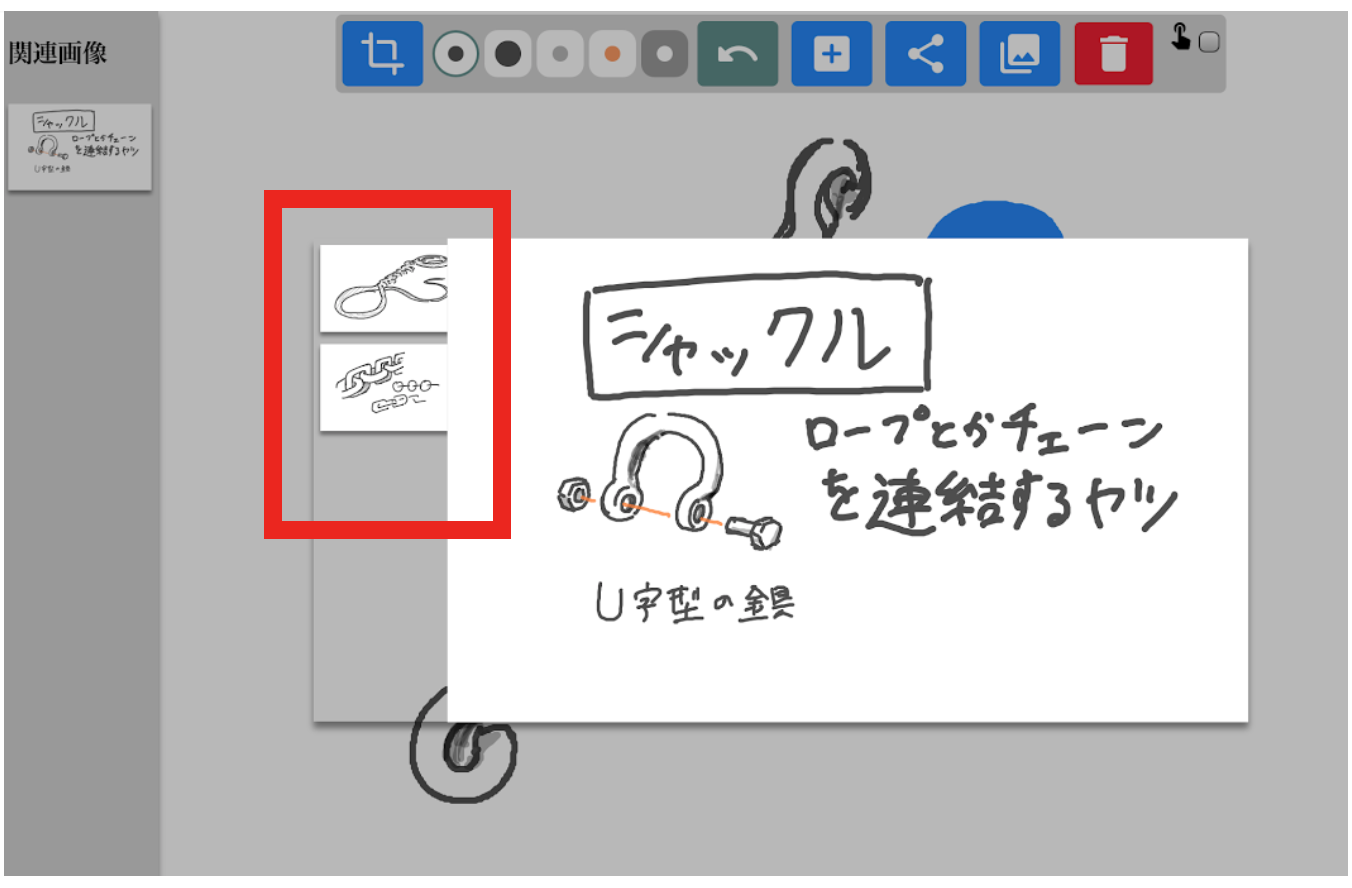
\includegraphics[width=70mm]{images/2hoplinkdialog.png}}
                   \end{center} \caption{関連画像のダイアログ} \label{fig:linkedIllust2}
\end{minipage}
\end{figure}

エディタの横に位置する"関連画像ビュー"には、
\begin{itemize}
    \item 現在表示中のメモ・イラストがリンクしている画像
    \item 現在表示中のメモ・イラストをリンクしている別のメモ・イラスト
\end{itemize}等のリンクに基づいた関連画像のサムネイルが表示される(図\ref{fig:linkedIllust1})。
また、サムネイルを選択するとリンクされている要素が強調表示され、対応関係が可視化される。
さらにリンク付要素をクリックすると、リンク先の画像がダイアログで表示される(図\ref{fig:linkedIllust2})。
このダイアログの内部にも関連画像ビューが内蔵されているため、現在表示している手書きメモ・イラストから最大2ホップで到達できる
メモやイラストを関連画像としてその場で参照することができる。
このようにリンクに基づいて関連するイラストを表示し、参照可能にする仕組みが備わっている。

\subsubsection{エキスポート・共有機能}

\begin{figure}[htbp] \begin{minipage}{0.5\hsize}
                         \begin{center} \fbox {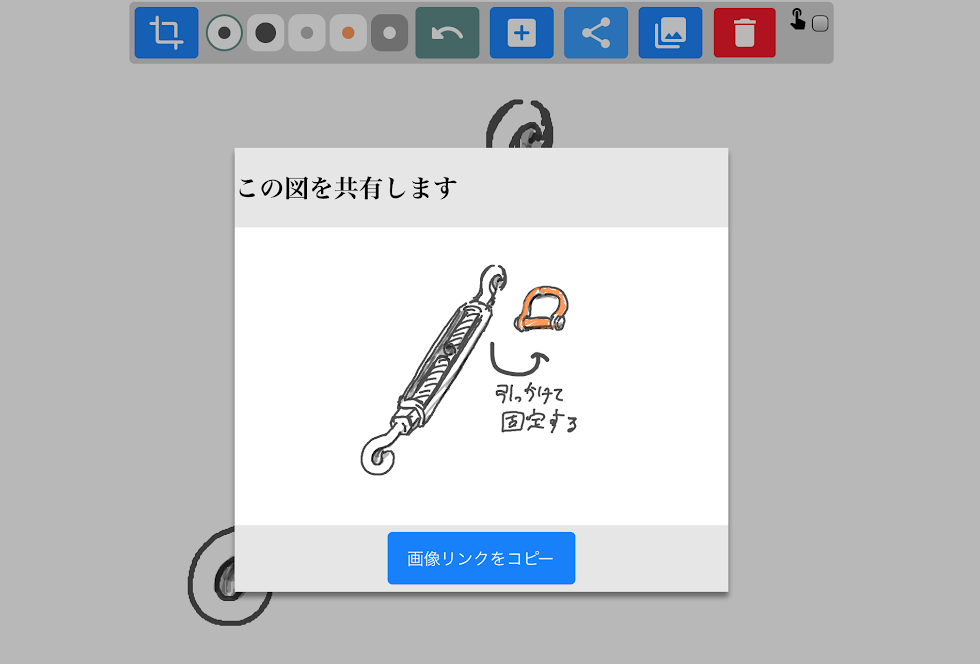
\includegraphics[width=70mm]{images/export1.png}}
                         \end{center} \caption{エキスポート機能の操作画面} \label{fig:exporting1}
\end{minipage} \begin{minipage}{0.5\hsize}
                   \begin{center} \fbox {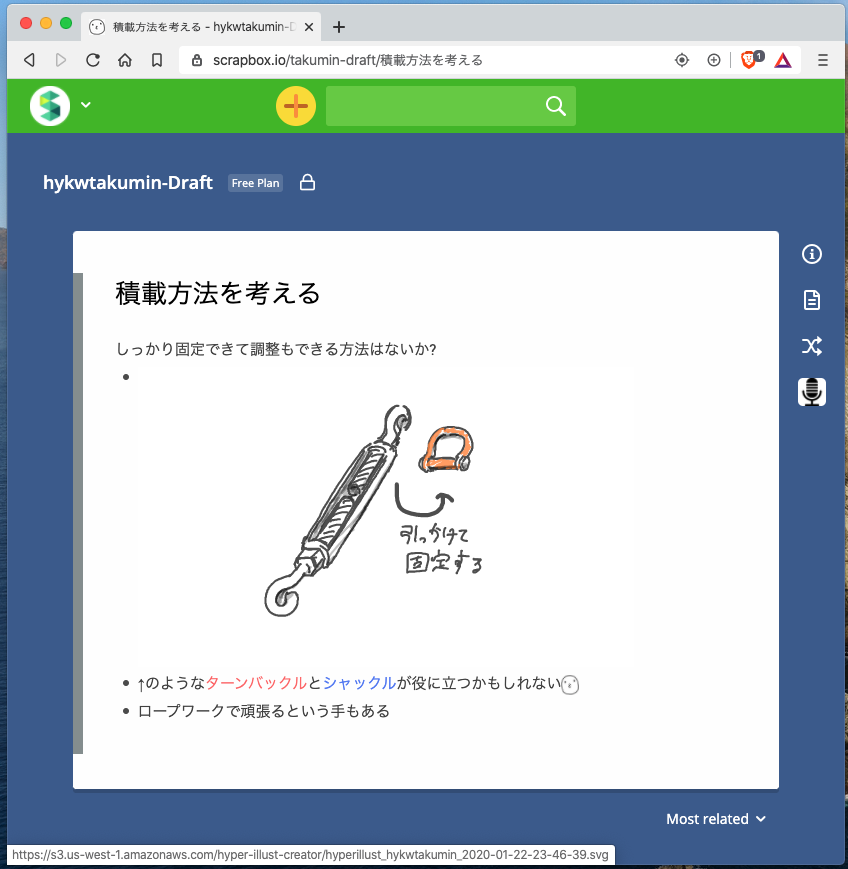
\includegraphics[width=70mm]{images/export2.png}}
                   \end{center} \caption{Webページに埋め込まれた手書きメモ} \label{fig:exporting2}
\end{minipage}
\end{figure}
エキスポート機能を利用すると、手書きメモ・イラストのファイルそのもの(SVG)のURLを取得することができる。
このURLをimg要素\footnote{https://developer.mozilla.org/ja/docs/Web/HTML/Element/img}やiframe要素\footnote{https://developer.mozilla.org/ja/docs/Web/HTML/Element/iframe}のsrc属性や
Object要素\footnote{https://developer.mozilla.org/ja/docs/Web/HTML/Element/object}のdata属性に指定することが可能で、
図\ref{fig:exporting2}のように他のWebサイトにも埋めこんで利用することができる。
画像としてエキスポートした状態でも埋め込んだハイパーリンクは有効であり、埋め込まれた要素をクリックすることでリンクされた別のメモや関連画像にアクセスすることができる。


\subsubsection{画像一覧機能}

\begin{figure}[htbp]
    \begin{center}
    {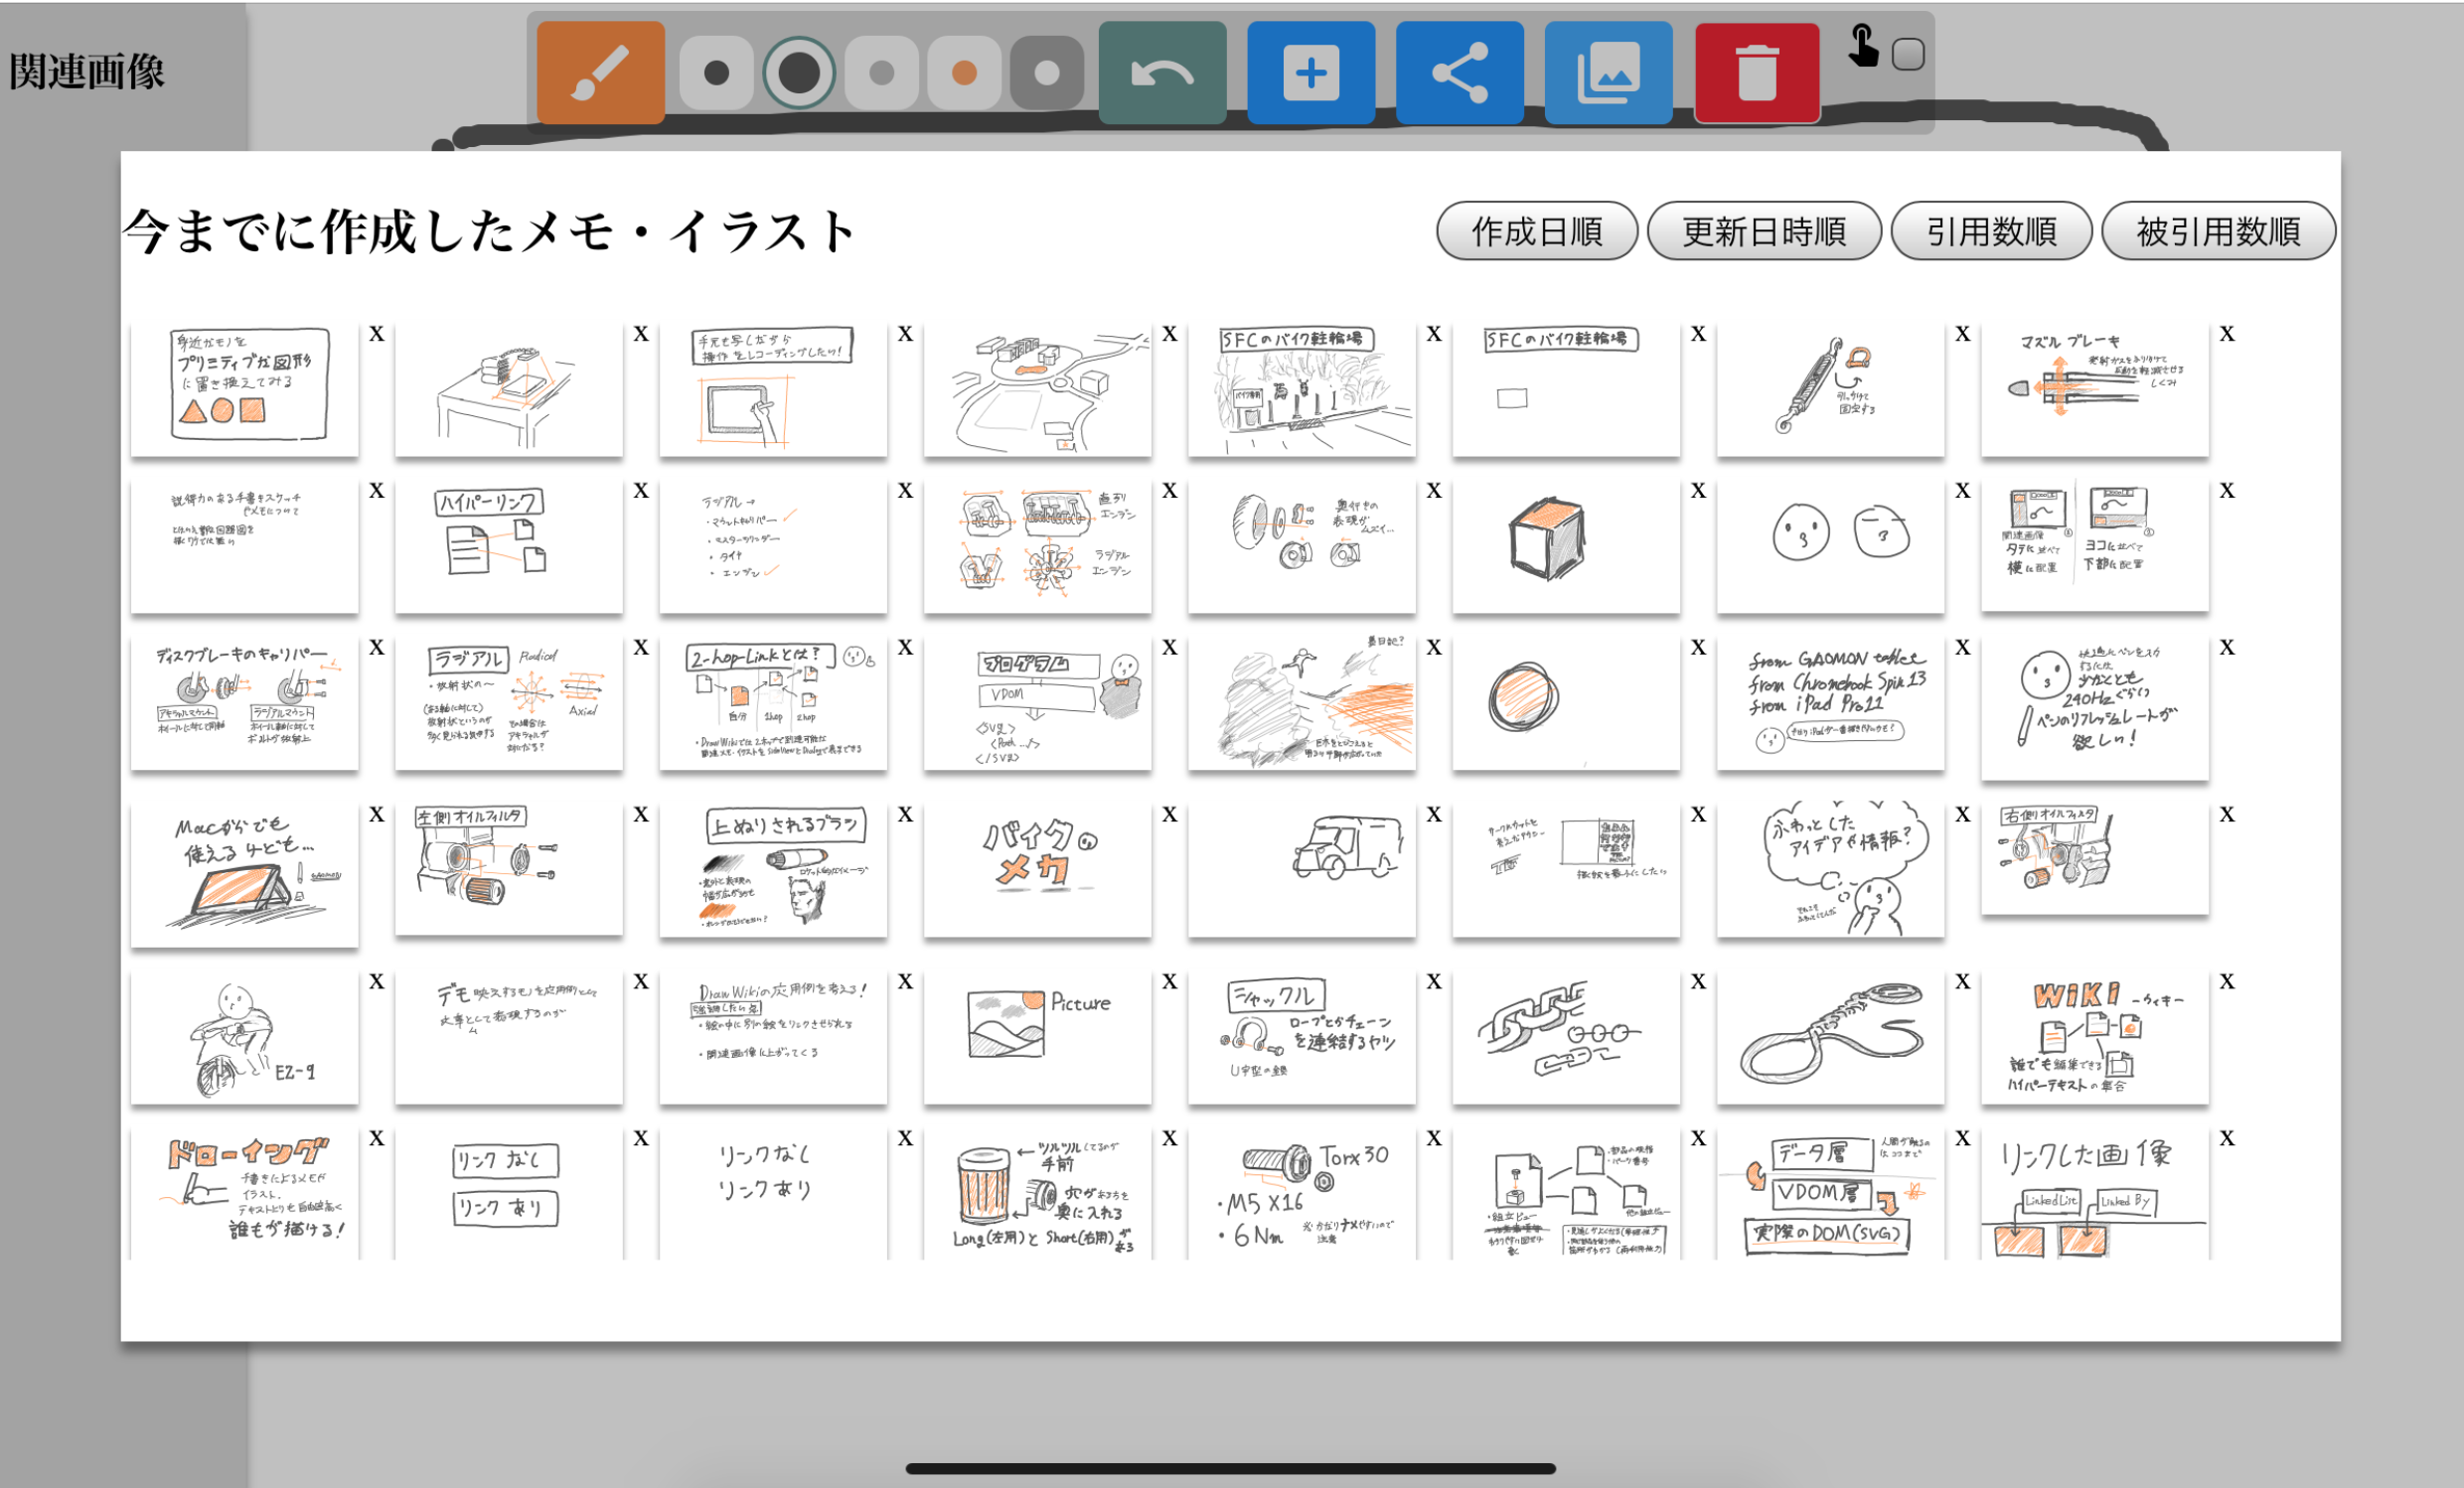
\includegraphics[width=100mm]{images/drawwikiimagelist.png}} \end{center}
    \caption{既存の画像を表示する画面}
    \label{imagelistview}
\end{figure}

DrawWikiで作成した画像は一覧画面から表示することができる。デフォルトでは画像の更新日時順に表示しているが、
作成日順、引用数順、被引用数順にソートすることもできる。引用数順では多くのメモ・イラストをリンクしているハブ的な役割を持つ画像が、
被引用数順では多くのメモ・イラストからリンクされている汎用性の高い画像が優先的に表示される。